 
\def\filename{leaflet-manual.tex}
\def\fileversion{v1.0d}   % change this when leaflet-manual changed, too.
\def\filedate{2012/06/04}
\def\docdate {2012/06/04} % change this when leaflet-manual changed, too.
\listfiles
\errorcontextlines=99
\documentclass[
notumble,
nofoldmark,
%%dvipdfm,
%%portrait,
%%titlepage,
%%nocombine,
%%a3paper,
%%debug,
%%nospecialtricks,
%%draft,
]{leaflet}
\usepackage{tabularx}
\usepackage{lipsum}
\usepackage{eurosym}
\renewcommand*\foldmarkrule{.3mm}
\renewcommand*\foldmarklength{5mm}

\usepackage[T1]{fontenc}
% \usepackage[T3]{inputenc}
\usepackage{textcomp}
\usepackage{mathptmx}
\usepackage{libertine}
\usepackage[scaled=0.9]{helvet}
\makeatletter
\def\ptmTeX{T\kern-.1667em\lower.5ex\hbox{E}\kern-.075emX\@}
\DeclareRobustCommand{\ptmLaTeX}{L\kern-.3em
        {\setbox0\hbox{T}%
         %\vb@xt@ % :-)
         \vbox to\ht0{\hbox{%
                            \csname S@\f@size\endcsname
                            \fontsize\sf@size\z@
                            \math@fontsfalse\selectfont
                            A}%
                      \vss}%
        }%
        \kern-.12em
        \ptmTeX}
\makeatother
\let\TeX=\ptmTeX
\let\LaTeX=\ptmLaTeX
\usepackage{shortvrb}
\MakeShortVerb{\|}
\usepackage{url}
\usepackage{graphicx}
\usepackage[dvipsnames,usenames]{color}
\definecolor{LIGHTGRAY}{gray}{.9}
\definecolor{lspblue1}{cmyk}{0.9,0.4,0.05,0}
\usepackage{langscicolors}
%%%%\renewcommand{\descfont}{\normalfont}
\newcommand\Lpack[1]{\textsf{#1}}
\newcommand\Lclass[1]{\textsf{#1}}
\newcommand\Lopt[1]{\texttt{#1}}
\newcommand\Lprog[1]{\textit{#1}}

\newcommand*\defaultmarker{\textsuperscript\textasteriskcentered}

\title{The document class \Lclass{leaflet}}
\author{%
  Rolf Niepraschk\\
  Walter Schmidt\\
  Hubert G\"a\ss lein}
\date{Last updated~\docdate\\printed \today}

\CutLine*{1}% Dotted line without scissors
\CutLine*{6}%   

% \AddToBackground{5}{%  Background of a small page
%   \put(0,0){\textcolor{Cerulean}{\rule{\paperwidth}{\paperheight}}}}
\AddToBackground*{1}{%  Background of a small page
  \put(0,0){\textcolor{lspblue1}{\rule{\paperwidth}{\paperheight}}}}
\AddToBackground*{2}{%  Background of a small page
  \put(0,0){\textcolor{lspblue1}{\rule{\paperwidth}{\paperheight}}}}

% \AddToBackground*{2}{% Background of a large page
%   \put(\LenToUnit{.5\paperwidth},\LenToUnit{.5\paperheight}){%
%     \makebox(0,0)[c]{%
%       \resizebox{.9\paperwidth}{!}{\rotatebox{35.26}{%
%         \textsf{\textbf{\textcolor{LIGHTGRAY}{BACKGROUND}}}}}}}}

\AddToBackground{2}{
    \put(-2,580){
        
\includegraphics[width=3\paperwidth]{lsp-rainbow-large.png}%
%  \setlength{\tabcolsep}{0pt}
% 	\begin{tabularx}{3\paperwidth}{X|X|X|X|X|X|X|X|X|X|X|X|X|X|X|X|X|X|X}
% &&&&&&&&&&&&&&&&&&
% \end{tabularx}
    } 
}

% \AddToBackground{5}{
%     \put(-2,-100){
%         
\includegraphics[width=3\paperwidth]{lsp-rainbow-large.png}%
% %  \setlength{\tabcolsep}{0pt}
% % 	\begin{tabularx}{3\paperwidth}{X|X|X|X|X|X|X|X|X|X|X|X|X|X|X|X|X|X|X}
% % &&&&&&&&&&&&&&&&&&
% % \end{tabularx}
%     } 
% }


\AddToBackground{6}{
    \put(280,0){
        
\includegraphics[width=1\paperwidth,height=3.5cm]{lsp-rainbow-large.png}%
    } 
}

\AddToBackground{2}{
    \put(-2,10){
        
\includegraphics[width=.3\paperwidth]{lsp-rainbow-large.png}%
    } 
}

% \AddToBackground{3}{
%     \put(-2,10){
%         
\includegraphics[width=.3\paperwidth]{lsp-rainbow-large.png}%
%     } 
% }

% \AddToBackground{4}{
%     \put(-2,10){
%         
\includegraphics[width=.3\paperwidth]{lsp-rainbow-large.png}%
%     } 
% }


\begin{document}

% \maketitle
\thispagestyle{empty}

%%\LARGE
\color{LIGHTGRAY}
%%\tableofcontents
\noindent 
~
\parbox{.1\paperwidth}{
\vspace*{-.5cm}

\includegraphics[width=.3\paperwidth]{langsci_logo_nocolor.pdf} 
}
\parbox{.8\paperwidth}{
\raggedleft 
\vspace*{-2.5cm}{
\includegraphics[width=.4\paperwidth]{lsp-rainbow-large.png}}
}

\vspace*{12cm}

\raggedleft{
\Huge\sffamily \mbox{Language Science Press}\\[.3em]
\LARGE\sffamily Open Access Monographs}
\raggedright 

 \newpage



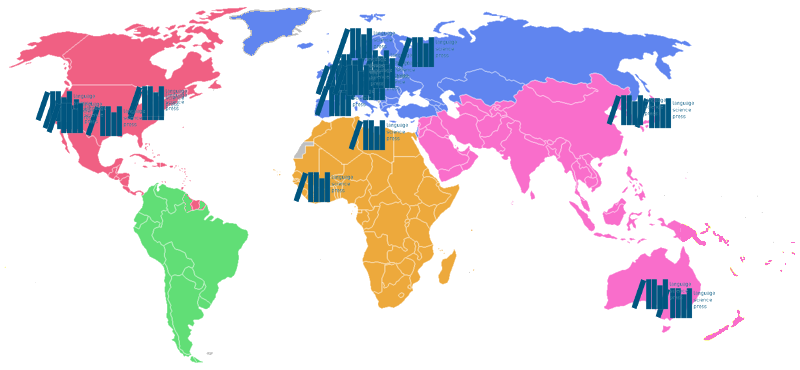
\includegraphics[width=2\textwidth]{worldmap.png}


\section{ \sffamily   \Large About}

High quality, peer-reviewed open-access books in linguistics

Free for both authors and readers

Published under a Creative Commons licence

General Editors are Stefan M\"uller (FU Berlin) and Martin Haspelmath (MPI for Evolutionary Anthropology)

Supported by a high-profile Advisory Board

Language Science Press is supported by the DFG with 500k\euro during the startup phase

Our philosophy is that book publishing can be fully under the control of scholars because most of the traditional tasks of commercial publishers can be done more efficiently by scholars

%     All books appear in a book series, and the series editors are responsible for acquiring, reviewing and selecting manuscripts for publication.
%     The authors are responsible for typesetting in LaTeX (together with the series editors); automatic conversion from Word is possible in principle.
%     The workflow is controlled by the publication management system OMP (Open Monograph Press).
%     Books are freely available in their PDF version; paper versions can be bought from print-on-demand companies.

% For some time now, all scholars have been accustomed to sharing their materials at no cost with their colleagues, often with the help of services like Academia.edu and ResearchGate. Scientific publication thus no longer serves the need of disseminating research results -- its purpose is to make the best work prominent enough to help build careers and to guide scholars in choosing what to read. This task of selecting the best work is carried out by the series editors of Language Science Press.

% To see published and forthcoming books, consult our catalogue. 
%Other pages of this site provide information for authors and information for series editors. We also provide templates for conversion from Word to LaTeX. The work of our volunteer supporters is appreciated in our Hall of Fame. Updates appear in our blog. 
 

\newpage 


\vspace*{8.9cm} 

For some time now, all scholars have been accustomed to sharing their materials at no cost with their colleagues, often with the help of services like Academia.edu and ResearchGate. Scientific publication thus no longer serves the need of disseminating research results -- its purpose is to make the best work prominent enough to help build careers and to guide scholars in choosing what to read. This task of selecting the best work is carried out by the series editors of Language Science Press.

Language Science Press is a scholar-owned press. We currently have 14 series with editorial board members from all over the world.
 
\newpage 

\section{ \sffamily \Large Series}

\newcommand{\leftseries}[3]{   
  \parbox{.1\textwidth}{~}
  \parbox{.7\textwidth}{\raggedleft\small #1\\{\scriptsize #3}}
  \parbox{.1\textwidth}{\includegraphics[width=.8cm]{#2.png}} 
}

\newcommand{\rightseries}[3]{   
  \parbox{.1\textwidth}{\includegraphics[width=.8cm]{#2.png}}
  \parbox{.7\textwidth}{\raggedright\small #1\\{\scriptsize #3}}
  \parbox{.1\textwidth}{~} 
}

\leftseries{African Language Grammars and Dictionaries}{algad}{Adams Bodomo, Ken Hiraiwa, Firmin Ahoua}
\rightseries{Computational Models of Language Evolution}{cmle}{Luc Steel, Remi van Trijp}

\leftseries{Conceptual Foundations of Language Science}{cfls}{Mark Dingemanse, Nick Enfield}
\rightseries{Contemporary African Linguistics}{cal}{Lee Bickmore, Akinbiyi Akinlabi}

\leftseries{Empirically Oriented Theoretical Morphology and Syntax}{eotms}{Stefan M\"uller, Berthold Crysmann, Laura Kallmeyer}
\rightseries{Implemented Grammars}{eotms-ig}{Stefan M\"uller, Berthold Crysmann, Laura Kallmeyer}

\leftseries{Language Variation}{lv}{John Nerbonne, Dirk Geeraerts}
\rightseries{\mbox{Monographs on Comparative Niger-Congo}}{mcnc}{Valentin Vydrin, Larry Hyman, Konstantin Pozdniakov, Guillaume Segerer, John Watters}

\leftseries{Studies in Caribbean Languages}{scl}{John R. Rickford, Joseph Farquharson}
\rightseries{Studies in Diversity Linguistics}{sidl}{Martin Haspelmath, Fernando Z\'u\~niga, Peter Arkadiev, Ruth Singer, Pilar Valenzuela}

\leftseries{Studies in Laboratory Phonology}{silp}{Martine Vrice, Doris M\"ucke, Taehong Cho}
\rightseries{Textbooks in Language Sciences}{tbls}{Stefan M\"uller, Martin Haspelmath, Claude Hag\`ege, Marianne Mithun, Anatol Stefanowitsch, Foong Ha Yap} 
 
\leftseries{Topics at the Grammar-Discourse Interface}{tgdi}{Philippa Cook, Anke Holler, Cathrine Fabricius-Hansen}
\rightseries{Translation and Multilingual Natural Language Processing}{tmnlp}{Reinhard Rapp, Silvia Hansen-Schirra, Oliver \v{C}ulo}
  
    
 

\newpage 
\color{LIGHTGRAY}
\section{ \sffamily \Large Advisory Board}

\begin{itemize}
 \item[$\rangle$] Artemis Alexiadou (Stuttgart)
 \item[$\rangle$] Jim Blevins ( Cambridge)
 \item[$\rangle$] Balthasar Bickel (Z\"urich)
 \item[$\rangle$] Geert Booij (Leiden)
 \item[$\rangle$] Miriam Butt (Konstanz)
 \item[$\rangle$] Ewa D\k{a}browska (Northumbria U)
 \item[$\rangle$] Arnulf Deppermann (IDS Mannheim)
 \item[$\rangle$] Nomi Erteschik-Shir (Ben Gurion)
 \item[$\rangle$] Martine Grice (U Cologne)
 \item[$\rangle$] Mutsumi Imai (Keio University)
 \item[$\rangle$] Laura Kallmeyer (D\"usseldorf)
 \item[$\rangle$] Manfred Krifka (Berlin)
 \item[$\rangle$] Mary Esther Kropp Dakubu (Ghana)
 \item[$\rangle$] Aditi Lahiri (Oxford)
 \item[$\rangle$] Stephen Levinson (MPI Nijmegen)
 \item[$\rangle$] Anke L\"udeling (Berlin)
 \item[$\rangle$] Detmar Meurers (T\"ubingen)
 \item[$\rangle$] Sam Mchombo (Berkeley)
 \item[$\rangle$] Rachel Nordlinger (Melbourne)
 \item[$\rangle$] Jairo Nunes (S�o Paulo)
 \item[$\rangle$] Steven Pinker (Harvard)
 \item[$\rangle$] Friedemann Pulverm\"uller (Berlin)
 \item[$\rangle$] Stuart Shieber (Harvard)
 \item[$\rangle$] Dieter Stein (D\"usseldorf)  
\end{itemize}

    
    
    
    
    
    
    
    
    
    
    
    
    
    
    
     
    
   
   
   
   
\newpage 

\section{ \sffamily \Large Support us!}
  
    \begin{itemize}
      \item[$\rangle$] submit your manuscript to one of the series
      \item[$\rangle$] become a community proofreader 
      \item[$\rangle$] become a community typesetter
      \item[$\rangle$] become a public supporter
      \item[$\rangle$] donate
    \end{itemize} 

\section{ \sffamily \Large Contact}
 

\includegraphics[width=.4\textwidth]{qrcode.eps}

{\LARGE \sffamily www.langsci-press.org}

{\LARGE \sffamily  contact@langsci-press.org}

Stefan M�ller, Martin Haspelmath (Press Directors)
Sebastian Nordhoff (Coordinator)

% \framebox[3cm]{ \textbf{Mitmachen?}\\ Author\par Editor}




% \fbox{
% \textbf{Mitmachen?}
% \\
% Author
% \\
% Editor
% \\
% Proofreader
% \\
% Typesetter
% \\
% Membership
% \\
% Donate
% 
% }

% \begin{itemize}
%  \item[$\rangle$] autor
% \item[$\rangle$] hrsg
% \item[$\rangle$] proofreader
% \end{itemize}
 

\loggingall
\end{document}
\endinput
%%
%% End of file `leaflet-manual.tex'.
